%! Author = mkeim
%! Date = 7/18/24

\section{RP1: Statistically Significant Detection of Linguistic Change} \label{sec:paper_kulkarni}
\subsection{Introduction} \label{subsec:kulkarni_introduction}

Kulkarni et al.\ (2015) explores the problem of detecting changes in word usage patterns over time.
They introduce methods to identify words that have undergone significant shifts in \emph{meaning}, usage \emph{frequency}, or \emph{context}.
This is achieved by analyzing historical corpora, which contain vast amounts of text data spanning multiple years or even centuries.
The study utilizes diverse datasets, including Twitter posts, Amazon product reviews, and Google Book Ngrams, to construct time series for individual words.\\
The research conducted by Kulkarni et al.\ exhibits a compelling alignment with our own research objectives,
specifically focusing on the identification of data voids characterized by shifting semantic meanings over time.
Their exploration into these linguistic shifts has revealed interesting insights, such as the evolution of the word `gay,'
which transitioned from being cheerful or dapper to signifying homosexual or lesbian aspect around the mid-20th century.
To achieve understanding of this phenomenon, they intend to study the following research questions.
\begin{itemize}
    \item \para{RQ1.} \emph{What methods can quantify the statistical relevance of observed changes in a word's usage across different time periods?}\\
    Kulkarni et al.’s study uses three technical methods to understand how words change over time: \emph{frequency} analysis, \emph{syntactic} analysis, and \emph{distributional} analysis.
    The frequency method tracks how often words are used, revealing spikes in usage when significant events occur, like how \emph{breaking news} data voids can create a surge in specific keywords.
    The syntactic method looks at changes in the grammatical roles of words, while the distributional method examines word co-occurrence patterns to see how word meanings shift.
    Their approach not only uncovers the dynamic nature of language but also highlights “data voids,” -- areas where terms have \emph{evolved}, become \emph{outdated}, or \emph{fragmented} in meaning.

    \item \para{RQ2.} \emph{Given that a word's usage has changed, how can the precise moment or period of this shift be determined?}\\
    Understanding data voids involves not only recognizing that a change is occurring but also analyzing the specifics of how that change unfolds over time.
    It’s crucial to pinpoint not just the fact that a shift has happened, but also the exact moment when it took place.
    Kulkarni et al.\ tackle this challenge by implementing a \emph{change point detection algorithm} based on the \emph{Mean Shift} model.
    This method determines whether a word has experienced a significant shift and, if so, identifies the precise point at which this change occurred.
\end{itemize}

Next two sections, \Cref{subsec:kulkarni-rq1} and \Cref{subsec:kulkarni-rq2} focuses on the two research questions that this paper is studying, the approach they took to study and their results.

\subsection{What methods can quantify the statistical relevance of observed changes in a word's usage across different time periods?} \label{subsec:kulkarni-rq1}

\para{Overview.}
The challenge is to identify how the meaning of words changes over time.
To address this, they examine a corpus containing data from various domains like books, tweets, and reviews, known as the Temporal Corpus $(C)$ which spans over a time period $(S)$.
This corpus is divided into smaller segments called snapshots $C_t$, each of length $P$.
From these snapshots, a common vocabulary $V$ is created having words which are common across all snapshots.
To analyze changes in these words, a time series $T(w)$ is constructed for each word $w\in V$.
Kulkarni et al.\ propose several methods to create this time series, aimed at understanding the evolution of words over time.

\begin{figure}[!h]
    \centering
    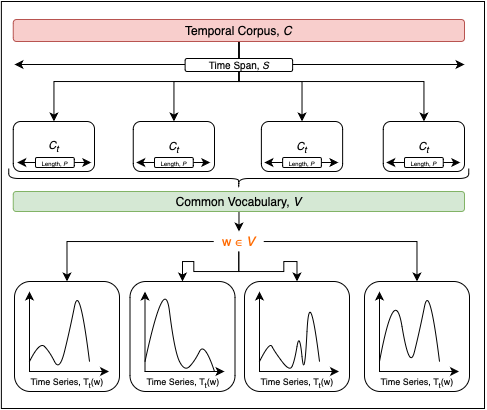
\includegraphics[scale=0.5]{figures/kulkarni1}
    \caption{My caption}
    \label{fig:label}
\end{figure}

\para{Construction of Time Series.}
In this paper, three methods are explored for statistically modeling the evolution of words over time:
frequency analysis, part-of-speech tagging, and word co-occurrence to create time series for each word.

\textbf{(1) Frequency-based method}: The simplest and most direct method for detecting sudden changes in word usage is by analyzing frequency trends.
\begin{wrapfigure}{R}{0.25\textwidth}
    \centering
    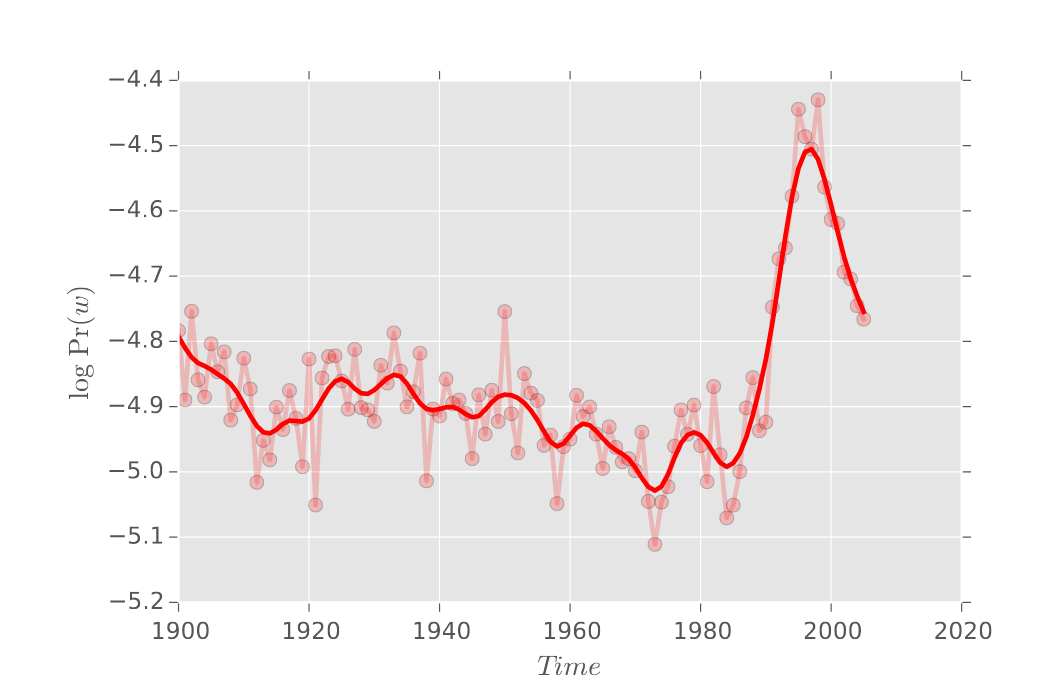
\includegraphics[width=0.25\textwidth]{figures/frequency-gay}
    \caption{My caption}
    \label{fig:example-gay}
\end{wrapfigure}

This approach examines how often a word is used over a given period, providing insights into shifts in its popularity or relevance.
Changes in frequency can indicate whether a word is gaining new meanings or losing old ones, reflecting broader cultural or societal trends.\\
For example, the word “gay” in \Cref{fig:example-gay} shows a noticeable spike in usage during the 1980s, signaling a shift in its meaning or cultural relevance.
Tools such as the Google Books Ngram Viewer and Google Trends are used for this purpose, as they provide large datasets and visual representations of word usage across different timeframes.
They calculate the change in probability of a word appearing over time.
\begin{displaymath}
$T_t(w) = \log \frac{#(w \in C_t)}{|C_t|}$ \label{eq:equation}
\end{displaymath}

\textbf{(2) Syntactic method:}
Frequency-based metrics, while simple to compute, are susceptible to errors caused by imbalances in the corpus's domain and genre distribution.
Fluctuations in word usage due to temporal events or the popularity of specific entities can obscure genuine shifts in word meaning.
Moreover, a word's grammatical role can evolve over time, such as acquiring a different part of speech category.
To study this, the corpus is annotated with part-of-speech (POS) tags, and the probability distribution of these tags is calculated for each word across different time snapshots.
This approach allows researchers to observe how a word’s syntactic role changes over time.

\textbf{(3) Distributional method}:
For detecting subtle semantic changes, which are not changed either due to frequency or through change in part of speech,
this method was developed to understand in which context a word is used in and based on that understand the semantic changes.
Distributional methods focusses on creating a semantic space that maps words to continuos vector space, where each word is represented by a vector.
Once they created a temporal word embeddings for each word in each time snapshot, then they track the changes of the represtantations across the embedding space.

\begin{itemize}
    \item The researchers aimed to \emph{learn word embeddings} by training neural language models on a corpus at different time snapshots.
        They initialized word vector representations randomly and optimized the model parameters using stochastic gradient descent.
        During training, the objective was to maximize the probability of context words appearing around a target word.
        After training, word embeddings were normalized by their L2 norm to ensure consistent representation.
    \item The \emph{alignment} process involved aligning word embeddings from different time snapshots into a unified coordinate system to characterize changes between them.
        Assumptions were made to aid the alignment process, including the equivalence of spaces under linear transformation and the preservation of local structure of most words over time.
        When the alignment model failed to align a word correctly, it indicated a potential linguistic shift, highlighting the importance of accurate alignment for tracking semantic changes over time.
    \item By aligning embedding spaces across various time snapshots into a joint embedding space,
        the distributional method constructs a \emph{distributional time series} that captures the semantic evolution of words over time.
    \item The paper shows the evolution of the word `tape' over time.
        Initially, the word `tape' referred to an `adhesive tape' but underwent a semantic shift to also mean a `cassette tape' during the early 1970s.
\end{itemize}

\subsection{Given that a word's usage has changed, how can the precise moment or period of this shift be determined?} \label{subsec:kulkarni-rq2}
After constructing time series data for each word in the corpus—whether using frequency-based, syntactic, or distributional methods—the next step is to determine if the word has experienced a significant change.
If a significant shift is detected, the algorithm then identifies and returns the estimated change point (ECP), which marks the time when this change occurred.
\begin{itemize}
    \item Since language exhibits a stochastic drift.
        In this context, `stochastic' refers to the randomness or probabilistic nature of the training process,
        where the models are trained on the same dataset but may produce different results each time due to this randomness.
        To resolve this, time series was normalized for each word by transforming the time series into a Z-score series.
    \item Then the algorithm utilizes a Mean Shift model to detect changes in the mean of the time series.
    \item Change points can be thus identified by detecting significant shifts in the mean.
\end{itemize}

\subsection{Results} \label{subsec:kulkarni-results}

\para{Time Series Analysis \& Historical Analysis.} \\

\begin{table}[]
\begin{tabular}{@{}lllll@{}}
\toprule
\textbf{Method}         & \textbf{Examples}                              &  &  &  \\ \midrule
\textbf{Frequency}      & transmistted, bitch, sex, her                  &  &  &  \\
\textbf{Syntactic}      & apple, hug, sink, click, handle, windows, bush &  &  &  \\
\textbf{Distributional} & diet, tape, plastic                            &  &  &  \\ \bottomrule
\end{tabular}\label{tab:time-series-examples}
\end{table}

Frequency \& Distributional - transmistted, bitch, sex, her
The sharp increase of the word her in frequency around the 1960’s could be attributed to the concurrent rise and popularity of the feminist movement.
Sudden temporary popularity of specific social and political events could lead the Frequency method to produce many false positives.

Syntactic - apple, hug, sink, click, handle, windows, bush
The word apple was detected uniquely by the Syntactic method as its most frequent part of speech tag changed significantly from “Noun” to “Proper Noun”
The Syntactic method is indicative of having low false positive rate, but suffers from a high false negative rate, given that only two words in the table were detected.

Distributional - diet, tape, plastic
The popularity of books on dieting started with the best selling book Dr. Atkins’ Diet Revolution by Robert C. Atkins in 1972.
This changed the use of the word diet to mean a life-style of food consumption behavior and not only the food consumed by an individual or group.

\para{Cross Domain Analysis.}
Amazon Reviews and Twitter (content that spans a much shorter time scale as compared to Google Books Ngram Corpus)
What is the effect of applying distributional method on Amazon Review, Twitter dataset


\begin{table}[]
\begin{tabular}{@{}lllll@{}}
\toprule
\textbf{Dataset Source} & \textbf{Examples}                     &  &  &  \\ \midrule
\textbf{Amazon Reviews} & streaming, ray, combo, rays, twilight &  &  &  \\
\textbf{Twitter Tweets} & candy, myster, rally, sandy           &  &  &  \\ \bottomrule
\end{tabular}\label{tab:sources-examples}
\end{table}

Words - streaming, ray, combo, rays, twilight

Twitter - candy, myster, rally, sandy
The word sandy acquired a new sense after the incident of Hurricane Sandy hitting the East Coast of USA, which was also mentioned in the data voids example by danah boyd.

These examples show that their method can detect the introduction of new products, movies, and books.

\subsection{Takeaways} \label{subsec:kulkarni-takeaways}
The paper by Kulkarni et al.\ (2015) contributes a novel and rigorous approach to detecting linguistic changes using statistical methods and word embeddings.
Their contribution in using large historical corpora and word embeddings to capture the dynamic nature of language.
A statistical framework that ensures the detected changes are significant, avoiding false positives due to noise or minor fluctuations.

Despite the fast pace of change of the web content, our method is able to detect the introduction of new products, movies and books. This could help semantically aware web applications to better understand user intentions and requests.


%Also, after knowing that a change has occurred, we would like to know when did that change really occur so that we can co-relate that the data void occured when a political event happened or how the COVID outbreak event,
%which could help us identify that the term were introduced due to that event, which can be a future direction we can look into.

%For example, the term "filmyourhospital" was introduced in during 2020 when coronavirus took place, which corresponds to a sudden spike.
%And this term was never used before 2020, making it a new term that introduced to support the conspiracy theory regarding encouraged people to visit local hospitals to take pictures and videos of empty hospitals to help “prove” that the COVID-19 pandemic is an elaborate hoax.
%Correlate with historical events.
